\begin{frame}
  \frametitle{3D Point to Pixel: Estimating the Parameters of P}
  \begin{equation*}
    \underset{\substack{\text{pixel}\\ \text{coordinate}}}{\vec{x}} \sim \underset{\substack{\text{trans-}\\ \text{formation}}}{\vec{P}}
    \underset{\substack{\text{world}\\ \text{coordinate}}}{\vec{X}}
  \end{equation*}  
\end{frame}

\begin{frame}
  \frametitle{Estimating Camera Parameters Given the Geometry}
  \begin{itemize}
    \item known control points
  \end{itemize}
  \begin{center}
    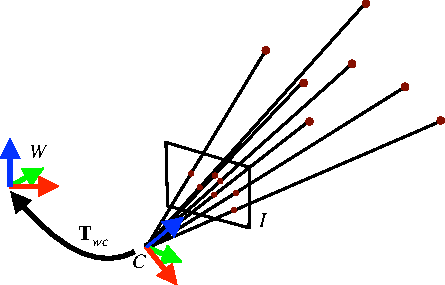
\includegraphics[width=0.5\columnwidth]{./images/dlt_3d_2d.pdf}
  \end{center}
\end{frame}

\begin{frame}
  \frametitle{Estimate Ex- and Intrinsics}
  \begin{itemize}
    \item \textbf{Wanted}: Extrinsic and intrinsic parameters of a camera
    \item \textbf{Given}: Coordinates of object points (control points)
    \item \textbf{Observed}: Coordinates of those known 3D object points in the image
  \end{itemize}
\end{frame}

\begin{frame}
  \frametitle{Mapping}
  Direct linear transform (DLT) maps any object point $\vec{X}$ to the image point $\vec{x}$.
  \begin{center}
    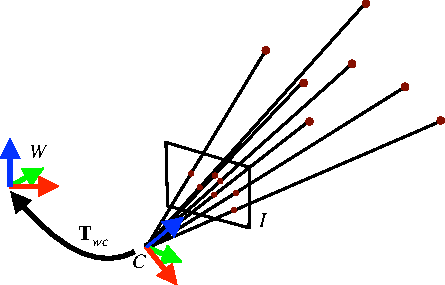
\includegraphics[width=0.5\columnwidth]{./images/dlt_3d_2d.pdf}
  \end{center}
%
  \begin{equation*}
    \vec{x} = \projectionMatrix \vec{X} \quad \text{donde} \quad
    \underset{3 \times 4}{\projectionMatrix}=\underset{3 \times 3}{\intrinsicMatrix}\underset{3 \times 4}{\begin{bmatrix} \underset{3 \times 3}{\rotation} & \underset{3 \times 1}{\translation}\end{bmatrix}}
  \end{equation*}
%
\end{frame}

% \begin{frame}
%   \frametitle{Camera Parameters}
%   \begin{itemize}
%     \item Intrinsics -- Camera-internal parameters. Given through $\intrinsicMatrix$.
%     \item Extrinsics -- Pose parameters of the camera. Given through $\rotation$ and $\vec{X}_{0}$.
%     \item Projection matrix $\projectionMatrix$ contains both, the in- and extrinsics.
%   \end{itemize}

%   \begin{align*}
%     \vec{x} &= \projectionMatrix \vec{X}\\
%     \vec{x} &= \intrinsicMatrix \begin{bmatrix} \rotation & \translation \end{bmatrix} \vec{X}\\
%     \vec{x} &= \intrinsicMatrix \rotation \begin{bmatrix} \vec{I} & -\vec{X}_{0} \end{bmatrix} \vec{X}\\
%   \end{align*}
% \end{frame}

\begin{frame}
  \frametitle{Compute the 11 intrinsic and extrinsic parameters}
  Direct Linear Transform (DLT)
  \begin{itemize}
    \item control point coordinates (given)
    \item observed image point  (given)
    \item 3 rotations, 3 translations
    \item 5 intrinsic parameters $(f_{x}, f_{y}, \principalPoint_{x}, \principalPoint_{y}, s)$
  \end{itemize}

  \begin{center}
    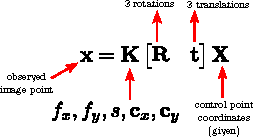
\includegraphics[width=0.5\columnwidth]{./images/projection_matrix_unknowns.pdf}
  \end{center}
\end{frame}

\begin{frame}
  \frametitle{How Many Points Are Needed?}

  \only<1-3>{
    
    Each point gives \alert{???} observation equations.

    \begin{equation*}
      \vec{x} = \projectionMatrix \vec{X}
    \end{equation*}
  }
  \only<2>{
    \begin{equation*}
      \begin{bmatrix} u\\ v\\ w\end{bmatrix} = \projectionMatrix \begin{bmatrix} U\\ V\\ W \\ T\end{bmatrix}
    \end{equation*}
  }

  \only<3>{
    \begin{equation*}
      \begin{bmatrix} \frac{u}{w}\\ \frac{v}{w}\\ 1\end{bmatrix} = \projectionMatrix \begin{bmatrix} \frac{U}{T}\\ \frac{V}{T}\\ \frac{W}{T} \\ T\end{bmatrix}
    \end{equation*}
  }

  \only<4>{
    \begin{equation*}
      \begin{bmatrix} x\\ y\\ 1\end{bmatrix} = \projectionMatrix \begin{bmatrix} X\\ Y\\ Z \\ 1\end{bmatrix}
    \end{equation*}


    \begin{align*}
      x &= \frac{p_{11}X + p_{12}Y + p_{13}Z + p_{14}}{p_{31}X + p_{32}Y + p_{33}Z + p_{34}}\\
      y &= \frac{p_{21}X + p_{22}Y + p_{23}Z + p_{24}}{p_{31}X + p_{32}Y + p_{33}Z + p_{34}}
    \end{align*}

    Each point gives \alert{two} observation equations, one for each image coordinate.
  }
\end{frame}

\begin{frame}
  \frametitle{Spatial Resection (P3P) vs. DLT}
  \begin{itemize}
    \item Calibrated camera: 
    \begin{itemize}
      \item 6 unknowns.
      \item Need at least 3 points.
      \item Problem solved by spatial resection
    \end{itemize}
    \item Uncalibrated camera: 
    \begin{itemize}
      \item 11 unknowns.
      \item Need at least 6 points 
      \item Assuming the model of an affine camera
      \item Problem solved by DLT
    \end{itemize}.
  \end{itemize}
\end{frame}

\begin{frame}
  \frametitle{DLT: Direct Linear Transform}
  Computing the Orientation of an Uncalibrated Camera using $\ge 6$ known points.
\end{frame}

\begin{frame}
  \frametitle{DLT: Problem Specification}
  \begin{itemize}
    \item Task: Estimate the 11 elements of $\projectionMatrix$.
    \item Given: 
    \begin{itemize}
      \item 3D coordinates $\vec{X}_{i}$ of object points.
      \item Observed image coordinates $\vec{x}_{i}$ of an uncalibrated camera with the mapping.
      \begin{equation*}
        \vec{x}_{i} = \projectionMatrix \vec{X}_{i} \quad i=1,\ldots,n \quad n \ge 6
      \end{equation*}
    \end{itemize}
    \item Data association
  \end{itemize}

\end{frame}

\begin{frame}
  \frametitle{Rearrange the DLT Equation}
  
  \only<1>{
    \begin{equation*}
      \vec{x}_{i} = \underset{3\times4}{\projectionMatrix} \vec{X}_{i} =
      \begin{bmatrix}
        p_{11} & p_{12} & p_{13} & p_{14} \\
        p_{21} & p_{22} & p_{23} & p_{24} \\
        p_{31} & p_{32} & p_{33} & p_{34}
      \end{bmatrix} \vec{X}_{i}
    \end{equation*}
  }

  \only<2->{
    \begin{equation*}
      \vec{x}_{i} = \underset{3\times4}{\projectionMatrix} \vec{X}_{i} =
      \begin{bNiceMatrix}[margin] 
        p_{11} & p_{12} & p_{13} & p_{14} \\
        p_{21} & p_{22} & p_{23} & p_{24} \\
        p_{31} & p_{32} & p_{33} & p_{34}
      \CodeAfter
        \tikz \node [draw=red, rounded corners, fit = (1-1) (1-last)] { } ;
        \tikz \node [draw=blue, rounded corners, fit = (2-1) (2-last)] { } ;
        \tikz \node [draw, rounded corners, fit = (3-1) (3-last)] { } ; 
      \end{bNiceMatrix} \vec{X}_{i}
    \end{equation*} 
  }
  \only<3>{
    Define the three vectors A, B and C as follows

    \begin{equation*}
      {\color{red} \boxed{\color{black}{\vec{A}}}} = \begin{bmatrix} p_{11}\\ p_{12}\\ p_{13}\\ p_{14} \end{bmatrix}, \quad
      {\color{blue} \boxed{\color{black}{\vec{B}}}} = \begin{bmatrix} p_{21}\\ p_{22}\\ p_{23}\\ p_{24} \end{bmatrix}, \quad
      \boxed{\vec{C}} = \begin{bmatrix} p_{31}\\ p_{32}\\ p_{33}\\ p_{34} \end{bmatrix}
    \end{equation*}
  }

  \only<4>{
    So what we can rewrite the equation as

    \begin{equation*}
      \vec{x}_{i} = \projectionMatrix \vec{X}_{i} =
      \begin{bNiceMatrix}[margin] 
        \vec{A}^{\top} \\
        \vec{B}^{\top} \\
        \vec{C}^{\top}
      \CodeAfter
        \tikz \node [draw=red, rounded corners, fit = (1-1) (1-last)] { } ;
        \tikz \node [draw=blue, rounded corners, fit = (2-1) (2-last)] { } ;
        \tikz \node [draw, rounded corners, fit = (3-1) (3-last)] { } ; 
      \end{bNiceMatrix} \vec{X}_{i}
    \end{equation*}
  }

  \only<5>{
    So what we can rewrite the equation as

    \begin{equation*}
      \begin{bmatrix}
        u_{i} \\
        v_{i} \\
        w_{i}
      \end{bmatrix} = 
      \vec{x}_{i} = \projectionMatrix \vec{X}_{i} =
      \begin{bNiceMatrix}[margin] 
        \vec{A}^{\top} \\
        \vec{B}^{\top} \\
        \vec{C}^{\top}
      \CodeAfter
        \tikz \node [draw=red, rounded corners, fit = (1-1) (1-last)] { } ;
        \tikz \node [draw=blue, rounded corners, fit = (2-1) (2-last)] { } ;
        \tikz \node [draw, rounded corners, fit = (3-1) (3-last)] { } ; 
      \end{bNiceMatrix} \vec{X}_{i} = 
      \begin{bmatrix}
        \vec{A}^{\top}\vec{X}_{i} \\
        \vec{B}^{\top}\vec{X}_{i} \\
        \vec{C}^{\top}\vec{X}_{i}
      \end{bmatrix}
    \end{equation*}
  }

\end{frame}

\begin{frame}
  \frametitle{Rearrange the DLT Equation}

  \begin{equation*}
    \vec{x}_{i} =
    \begin{bmatrix}
      x_{i} \\
      y_{i} \\
      1
    \end{bmatrix} =
    \begin{bmatrix}
      u_{i} \\
      v_{i} \\
      w_{i}
    \end{bmatrix} = 
    \begin{bmatrix}
      \vec{A}^{\top}\vec{X}_{i} \\
      \vec{B}^{\top}\vec{X}_{i} \\
      \vec{C}^{\top}\vec{X}_{i}
    \end{bmatrix}
  \end{equation*}

Implica

  \begin{equation*}
    x_{i} = \dfrac{u_{i}}{w_{i}} = \dfrac{\vec{A}^{\top}\vec{X}_{i}}{\vec{C}^{\top}\vec{X}_{i}}
    \quad \quad
    y_{i} = \dfrac{v_{i}}{w_{i}} = \dfrac{\vec{B}^{\top}\vec{X}_{i}}{\vec{C}^{\top}\vec{X}_{i}}
  \end{equation*}

\end{frame}

\begin{frame}
  \frametitle{Rearrange the DLT Equation}

  \begin{align*}
    x_{i} &= \dfrac{\vec{A}^{\top}\vec{X}_{i}}{\vec{C}^{\top}\vec{X}_{i}} \implies x_{i} \vec{C}^{\top}\vec{X}_{i} - \vec{A}^{\top}\vec{X}_{i} = 0\\
    y_{i} &= \dfrac{\vec{B}^{\top}\vec{X}_{i}}{\vec{C}^{\top}\vec{X}_{i}} \implies y_{i} \vec{C}^{\top}\vec{X}_{i} - \vec{B}^{\top}\vec{X}_{i} = 0
  \end{align*}

  Leads to a system of equation, which is linear in the parameters A, B and C

  \begin{equation*}
    \begin{matrix}
      -\vec{X}_{i}^{\top}\vec{A}& &+x_{i}\vec{X}_{i}^{\top}\vec{C} = 0 \\
      &-\vec{X}_{i}^{\top}\vec{B} &+y_{i}\vec{X}_{i}^{\top}\vec{C} = 0
    \end{matrix}  
  \end{equation*}

\end{frame}

\begin{frame}
  \frametitle{Estimating the Elements of $\projectionMatrix$}
  \begin{itemize}
    \item Collect elements of $\projectionMatrix$ into a parameter vector $\vec{p}$.
  \end{itemize}

  \begin{center}
    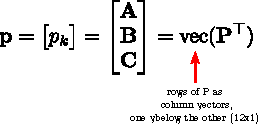
\includegraphics[width=0.5\columnwidth]{./images/projection_matrix_column_vector.pdf}
  \end{center}
  
\end{frame}

\begin{frame}
  \frametitle{Estimating the Elements of $\projectionMatrix$}
  \begin{itemize}
    \item Rewrite
    \begin{equation*}
      \begin{matrix}
        -\vec{X}_{i}^{\top}\vec{A}& &+x_{i}\vec{X}_{i}^{\top}\vec{C} = 0 \\
        &-\vec{X}_{i}^{\top}\vec{B} &+y_{i}\vec{X}_{i}^{\top}\vec{C} = 0
      \end{matrix}  
    \end{equation*}
      
    \item as
    \begin{align*}
        \vec{a}_{x_i}^{\top} \vec{p} &= 0 \\
        \vec{a}_{y_i}^{\top} \vec{p} &= 0
    \end{align*}

     \item with
    \begin{align*}
        \vec{p} &= (p_k) = \text{vec}(\vec{P}^{\top}) \\
        \vec{a}_{x_i}^{\top} &= \begin{bmatrix}-\vec{X}_i^{\top}, \vec{0}^{\top}, x_i \vec{X}_i^{\top}\end{bmatrix} \\
        &= \begin{bmatrix}-X_i, -Y_i, -Z_i, -1, 0, 0, 0, x_i X_i, x_i Y_i, x_i Z_i, x_i\end{bmatrix} \\
        \vec{a}_{y_i}^{\top} &= \begin{bmatrix}\vec{0}^{\top}, -\vec{X}_i^{\top}, y_i \vec{X}_i^{\top}\end{bmatrix} \\
        &= \begin{bmatrix}0, 0, 0, 0, -X_i, -Y_i, -Z_i, -1, y_i X_i, y_i Y_i, y_i Z_i, y_i\end{bmatrix}
    \end{align*}
  \end{itemize}
\end{frame}

% \begin{frame}
%   \frametitle{Verifying Correctness}
%   \begin{equation*}
%     \vec{a}_{x_i}^{\top} \vec{p} =
%     \begin{bmatrix}
%     -X_i, -Y_i, -Z_i, -1, 0, 0, 0, x_i X_i, x_i Y_i, x_i Z_i, x_i
%     \end{bmatrix}
%     \begin{bmatrix}
%     p_{11} \\
%     p_{12} \\
%     p_{13} \\
%     p_{14} \\
%     p_{21} \\
%     p_{22} \\
%     p_{23} \\
%     p_{24} \\
%     p_{31} \\
%     p_{32} \\
%     p_{33} \\
%     p_{34}
%     \end{bmatrix}  
%   \end{equation*}
  
% \end{frame}

% \begin{frame}
%   \frametitle{Verifying Correctness}
%   \begin{align*}
%     \vec{a}_{x_i}^{\top} \vec{p} &=
%     \begin{bmatrix}
%       -X_i, -Y_i, -Z_i, -1, 0, 0, 0, x_i X_i, x_i Y_i, x_i Z_i, x_i
%     \end{bmatrix}
%     \begin{bmatrix}
%       p_{11} \\
%       p_{12} \\
%       p_{13} \\
%       p_{14} \\
%       p_{21} \\
%       p_{22} \\
%       p_{23} \\
%       p_{24} \\
%       p_{31} \\
%       p_{32} \\
%       p_{33} \\
%       p_{34}
%     \end{bmatrix}\\
%     &= 
%     \begin{bmatrix}
%       \quad \quad \quad -\mathbf{X}_i^{\top},& \quad \quad \quad \mathbf{0},& \quad \quad \quad \quad x_i \mathbf{X}_i^{\top} \quad \quad \quad
%     \end{bmatrix}
%     \begin{bmatrix}
%     \mathbf{A} \\
%     \mathbf{B} \\
%     \mathbf{C}
%     \end{bmatrix} \\
%     &= \quad \quad \quad \quad -\mathbf{X}_i^{\top} \mathbf{A} \quad \quad \quad \quad \quad \quad \quad \quad+ x_i \mathbf{X}_i^{\top} \mathbf{C}
%   \end{align*}
% \end{frame}


\begin{frame}
  \frametitle{Verifying Correctness}

  \begin{center}
    \only<1>{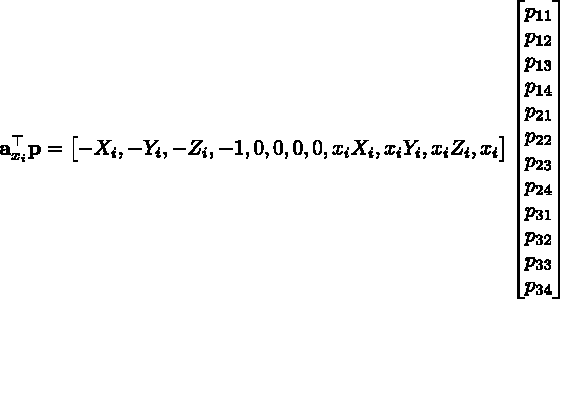
\includegraphics[width=0.7\columnwidth]{./images/verifying_correctness_1.pdf}}
    \only<2>{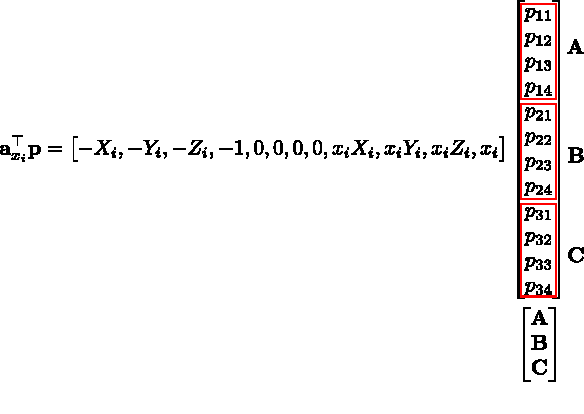
\includegraphics[width=0.7\columnwidth]{./images/verifying_correctness_2.pdf}}
    \only<3>{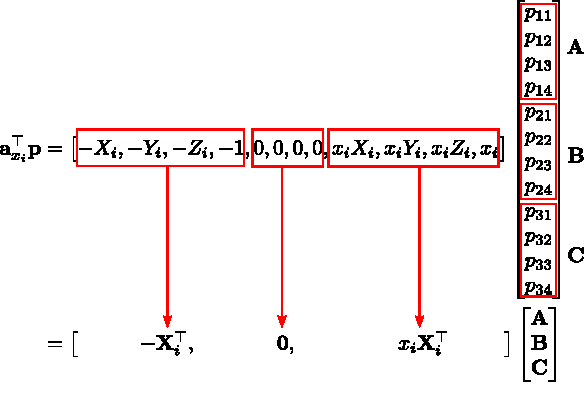
\includegraphics[width=0.7\columnwidth]{./images/verifying_correctness_3.pdf}}
    \only<4>{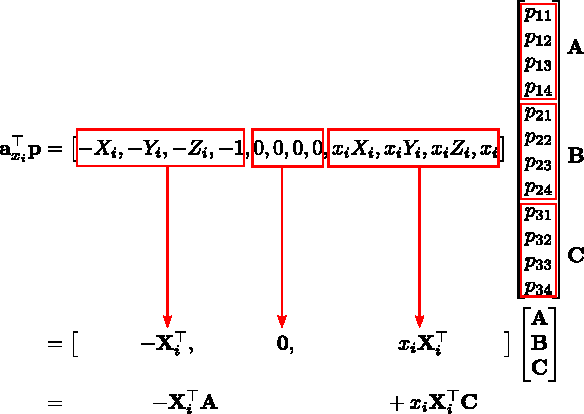
\includegraphics[width=0.7\columnwidth]{./images/verifying_correctness_4.pdf}}
    \only<5>{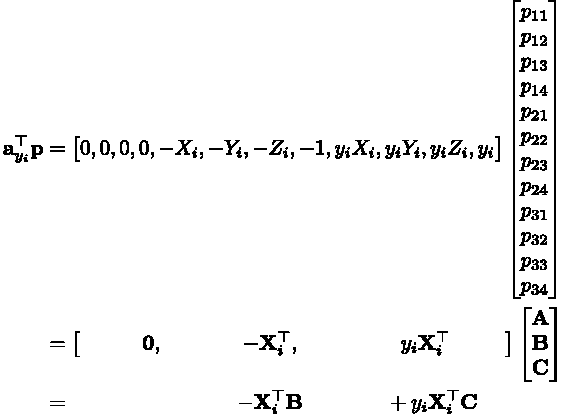
\includegraphics[width=0.7\columnwidth]{./images/verifying_correctness_5.pdf}}
  \end{center}

\end{frame}


\begin{frame}
  \frametitle{Estimating the Elements of P}

  \begin{itemize}
    \item For each point, we have
    \begin{align*}
        \vec{a}_{x_i}^{\top} \vec{p} &= 0 \\
        \vec{a}_{y_i}^{\top} \vec{p} &= 0
    \end{align*}
    \item Stacking everything together
    \begin{equation*}
      \begin{bmatrix}
        \vec{a}_{x_1}^{\top} \\
        \vec{a}_{y_1}^{\top} \\
        \vec{a}_{x_2}^{\top} \\
        \vec{a}_{y_2}^{\top} \\
        \vdots \\
        \vec{a}_{x_n}^{\top} \\
        \vec{a}_{y_n}^{\top}
      \end{bmatrix} \vec{p} = \underset{2I\times 12}{\vec{M}} \underset{12\times1}{\vec{p}} \stackrel{!}{=} 0
    \end{equation*}
  \end{itemize}

\end{frame}


\begin{frame}
  \frametitle{Solving the Linear System (Homogeneous System => SVD)}
  \begin{itemize}
    \item Solving a system of linear equations of the form $\vec{A}\vec{x} = \vec{0}$ is equivalent to finding the null space of $\vec{A}$
    \item Thus, we can apply the Singular value decomposition (SVD) to solve $\vec{M}\vec{p} = \vec{0}$
    \item Choose $\vec{p}$ as the singular vector belonging to the singular value of 0
  \end{itemize}
\end{frame}

\begin{frame}
    \frametitle{Redundant Observations}
    \begin{itemize}
        \item In case of redundant observations, we will have contradictions ($\vec{M}\mathbf{p} \neq \mathbf{0}$):
        %
        \begin{equation*}
            \mathbf{M} \mathbf{p} = \mathbf{w}
        \end{equation*}
        %
        \item Find $\mathbf{p}$ such that it minimizes
        %
        \begin{equation*}
            \Omega = \mathbf{w}^{\top} \mathbf{w}
        \end{equation*}
        \begin{align*}
            \implies \mathbf{\hat{p}} &= \underset{\mathbf{p}}{\arg\min} \ \mathbf{w}^{\top} \mathbf{w}\\
            &= \underset{\mathbf{p}}{\arg\min} \ \mathbf{p}^{\top} \mathbf{M}^{\top} \mathbf{M} \mathbf{p}
        \end{align*}
        \begin{equation*}
          \text{with} \lVert\mathbf{P}\rVert_2 = \sum_{i,j} p_{ij}^2 = \lVert\mathbf{p}\rVert = 1
        \end{equation*}
    \end{itemize}
\end{frame}


% --- Slide: Redundant Observations (2) ---
\begin{frame}
    \frametitle{Redundant Observations}
    \begin{itemize}
        \item Singular value decomposition (SVD)
        \[
            \mathbf{M}_{2I \times 12} = \mathbf{U}_{2I \times 12} \mathbf{S}_{12 \times 12} \mathbf{V}_{12 \times 12}^{\top} = \sum_{i=1}^{12} s_i \mathbf{u}_i \mathbf{v}_i^{\top}
        \]
        \item Choosing $\mathbf{p} = \mathbf{v}_{12}$ (the singular vector belonging to the smallest singular value $s_{12}$) minimizes $\Omega$
    \end{itemize}
\end{frame}

% --- Slide: Obtaining the Projection Matrix ---
\begin{frame}
    \frametitle{Obtaining the Projection Matrix}
    \begin{itemize}
        \item Choosing $\mathbf{p} = \mathbf{v}_{12}$ minimizes $\Omega$ and thus is our estimate of $\mathbf{P}$:
        \begin{equation*}
            \mathbf{p} = \begin{bmatrix}
            p_{11} \\
            \vdots \\
            p_{34}
            \end{bmatrix}
            \implies
            \mathbf{P} = \begin{bmatrix}
            p_{11} & p_{12} & p_{13} & p_{14} \\
            p_{21} & p_{22} & p_{23} & p_{24} \\
            p_{31} & p_{32} & p_{33} & p_{34}
            \end{bmatrix}
        \end{equation*}
    \end{itemize}
    \vspace{1cm}
    \centering
    \textcolor{red}{\bfseries Does this always work?}
\end{frame}

% --- Slide: Critical Surfaces (1 - The one with the note e.g.) ---
\begin{frame}
    \frametitle{Critical Surfaces}
    \begin{itemize}
        \item $\mathbf{M}$ is of rank 11, if
        \begin{itemize}
            \item Number of points $\geq 6$
            \item Assumption: no gross errors
        \end{itemize}
        \item \textcolor{red}{\bfseries No solution}, if all points $\mathbf{X}_i$ are located on a \textcolor{red}{\bfseries plane}
    \end{itemize}

    % The matrix part is complex due to the arrows, so we'll use a simplified aligned version
    \begin{align*}
      \mathbf{M} &= 
      \begin{bmatrix}
      \cdots \\
      \mathbf{a}_{x_i}^{\top} \\
      \mathbf{a}_{y_i}^{\top} \\
      \cdots
      \end{bmatrix}\\
      % The example row structure with arrows is very complex to code precisely,
      % but we can represent the key row structure.
      &=
      \begin{bmatrix}
          & & & & & \cdots & & & & & & \\
          -X_i & -Y_i & \color{red}{-Z_i} & -1 & 0 & 0 & 0 & 0 & x_i X_i & x_i Y_i & x_i \color{red}{Z_i} & x_i \\
          0 & 0 & 0 & 0 & -X_i & -Y_i & \color{red}{-Z_i} & -1 & y_i X_i & y_i Y_i & y_i \color{red}{Z_i} & y_i \\
          & & & & & \cdots & & & & & &
      \end{bmatrix}
    \end{align*}
    {\color{red} assume all $Z_{i} = 0$}
\end{frame}

% --- Slide: Critical Surfaces (2 - The one with the boxes/rank deficiency) ---
\begin{frame}
    \frametitle{Critical Surfaces}
    \begin{itemize}
        \item $\mathbf{M}$ is of rank 11, if
        \begin{itemize}
            \item Number of points $\geq 6$
            \item Assumption: no gross errors
        \end{itemize}
        \item \textcolor{red}{\bfseries No solution}, if all points $\mathbf{X}_i$ are located on a \textcolor{red}{\bfseries plane}
    \end{itemize}

    % The matrix part is complex due to the arrows, so we'll use a simplified aligned version
    \begin{align*}
      \mathbf{M} &= 
      \begin{bmatrix}
      \cdots \\
      \mathbf{a}_{x_i}^{\top} \\
      \mathbf{a}_{y_i}^{\top} \\
      \cdots
      \end{bmatrix}\\
      % The example row structure with arrows is very complex to code precisely,
      % but we can represent the key row structure.
      &=
      \begin{bNiceMatrix}[margin] 
        & & \phantom{0} & & & \cdots & \phantom{0} & & & & \phantom{0} & \\
        -X_i & -Y_i & 0 & -1 & 0 & 0 & 0 & 0 & x_i X_i & x_i Y_i & 0 & x_i \\
        0 & 0 & 0 & 0 & -X_i & -Y_i & 0 & -1 & y_i X_i & y_i Y_i & 0 & y_i \\
        & & \phantom{0} & & & \cdots & \phantom{0} & & & & \phantom{0} &
      \CodeAfter
        \tikz \node [draw=red, rounded corners, fit = (1-3) (4-3)] { } ;
        \tikz \node [draw=red, rounded corners, fit = (1-7) (4-7)] { } ;
        \tikz \node [draw=red, rounded corners, fit = (1-11) (4-11)] { } ; 
      \end{bNiceMatrix}
    \end{align*}
    {\color{red} assume all $Z_{i} = 0$}
\end{frame}

\begin{frame}
  \frametitle{Critical Surfaces}
  \begin{itemize}
      \item $M$ is of rank $11$, if
      \begin{itemize}
          \item Number of points $\geq 6$
          \item Assumption: no gross errors
      \end{itemize}
      \item \textbf{No solution}, if
      \begin{itemize}
          \item All points $X_i$ are located on a \textbf{plane}
          \item (All points $X_i$ and the projection center $X_O$ are located on a twisted cubic curve)
      \end{itemize}
  \end{itemize}
\end{frame}

\begin{frame}
  \frametitle{From $P$ to $K,R,t$}
  % \includegraphics[width=0.6\textwidth]{placeholder-image.jpg}
\end{frame}

\begin{frame}
  \frametitle{Decomposition of P}
  \begin{itemize}
    \item Compute $K, R, t$ from $P$.
    \item Use QR decomposition for rotation and calibration matrices.
  \end{itemize}
  % \includegraphics[width=0.7\textwidth]{placeholder-image.jpg}
\end{frame}


\begin{frame}
  \frametitle{Decomposition of P}
  \begin{itemize}
      \item We have $P$, how to obtain $K, R, X_O$?
      \item Structure of the projection matrix
      $$P = [KR \mid -KRX_O] = [H \mid \mathbf{h}]$$
      \item with
      $$H = KR \quad \mathbf{h} = -KRX_O$$
  \end{itemize}
\end{frame}

\begin{frame}
  \frametitle{Decomposition of P}

\end{frame}

\begin{frame}
  \frametitle{Decomposition of P}
  
\end{frame}

\begin{frame}
  \frametitle{Decomposition of P}
  
\end{frame}


\begin{frame}
  \frametitle{DLT in a Nutshell: Step 1}
    \begin{enumerate}
        \item \textbf{Build the matrix $M$ for the linear system} $\mathbf{M p} \stackrel{!}{=} \mathbf{0}$.
    \end{enumerate}
    \vspace{0.5cm}
    \begin{center}
        $M = \begin{bmatrix}
            \mathbf{a}_{x_1}^T \\
            \mathbf{a}_{y_1}^T \\
            \vdots \\
            \mathbf{a}_{x_l}^T \\
            \mathbf{a}_{y_l}^T
        \end{bmatrix}$
        \qquad
        $\underset{2l \times 12}{\mathbf{M}} \underset{12 \times 1}{\mathbf{p}} \stackrel{!}{=} \mathbf{0}$
        
        \vspace{0.5cm}
        with
        \begin{align*}
            \mathbf{a}_{x_i}^T &= (-X_i, -Y_i, -Z_i, -1, 0, 0, 0, 0, x_iX_i, x_iY_i, x_iZ_i, x_i) \\
            \mathbf{a}_{y_i}^T &= (0, 0, 0, 0, -X_i, -Y_i, -Z_i, -1, y_iX_i, y_iY_i, y_iZ_i, y_i)
        \end{align*}
    \end{center}
    \footnotesize{(Where $(X_i, Y_i, Z_i)$ are 3D world coordinates and $(x_i, y_i)$ are 2D image coordinates for control point $i$. $l$ is the number of control points.)}
\end{frame}

\begin{frame}
  \frametitle{DLT in a Nutshell: Step 2}
    \begin{enumerate}
        \setcounter{enumi}{1}
        \item \textbf{Solve by SVD} $\mathbf{M} = \mathbf{U} \mathbf{S} \mathbf{V}^T$.
    \end{enumerate}
    \vspace{0.5cm}
    \begin{center}
        The solution $\mathbf{p}$ is the \textbf{last column of $\mathbf{V}$}.
        \vspace{0.5cm}
        $$
        \mathbf{p} = \mathbf{v}_{12} \implies \mathbf{P} = \begin{bmatrix}
            p_1 & p_2 & p_3 & p_4 \\
            p_5 & p_6 & p_7 & p_8 \\
            p_9 & p_{10} & p_{11} & p_{12}
        \end{bmatrix}
        $$
        \footnotesize{($\mathbf{P}$ is the $3 \times 4$ projection matrix.)}
    \end{center}
\end{frame}

\begin{frame}
  \frametitle{DLT in a Nutshell: Step 3 (Decomposition)}
    \begin{enumerate}
        \setcounter{enumi}{2}
        \item \textbf{If individual parameters are needed}, decompose the projection matrix $\mathbf{P}$.
    \end{enumerate}
    \vspace{0.5cm}
    The projection matrix $\mathbf{P}$ can be written as:
    $$
    \mathbf{P} = \mathbf{K} \mathbf{R} [\mathbf{I}_3 | - \mathbf{X}_O] = [\mathbf{H} | \mathbf{h}]
    $$
    \begin{itemize}
        \item Camera center (Extrinsic translation): $\mathbf{X}_O = -\mathbf{H}^{-1} \mathbf{h}$
        \item The $3 \times 3$ matrix $\mathbf{H} = \mathbf{K} \mathbf{R}$ is the \textbf{calibration matrix} (Homography).
    \end{itemize}
    \vspace{0.5cm}
    Use $\mathbf{Q R}$ decomposition of $\mathbf{H}^{-1}$:
    $$
    \mathbf{Q R}(\mathbf{H}^{-1}) = \mathbf{R}^T \mathbf{K}^{-1}
    $$
    \vspace{0.5cm}
    \textbf{Normalization and Sign Ambiguity:}
    \begin{itemize}
        \item Due to homogeneity, \textbf{normalize} $\mathbf{K}$:
        $$
        \mathbf{K} \leftarrow \frac{1}{K_{33}} \mathbf{K}
        $$
        \item Decomposition $\mathbf{H}^{-1} = \mathbf{R}^T \mathbf{K}^{-1}$ results in $\mathbf{K}$ with \textbf{positive diagonal elements}.
        \item To get a \textbf{negative camera constant} (if desired, related to the sign of $c$ or $P$), apply:
        \begin{align*}
            \mathbf{K} &\leftarrow \mathbf{K} \mathbf{R}(z, \pi) \\
            \mathbf{R} &\leftarrow \mathbf{R}(z, \pi) \mathbf{R}
        \end{align*}
        using the rotation matrix:
        $$
        \mathbf{R}(z, \pi) = \begin{bmatrix}
            -1 & 0 & 0 \\
            0 & -1 & 0 \\
            0 & 0 & 1
        \end{bmatrix}
        $$
        \footnotesize{($\mathbf{P}$ is invariant under this transformation: $\mathbf{H} = \mathbf{K} \mathbf{R}(z, \pi) \mathbf{R}(z, \pi) \mathbf{R} = \mathbf{K} \mathbf{R}$.)}
    \end{itemize}
\end{frame}

\begin{frame}
  \frametitle{Discussion DLT}
    \begin{itemize}
        \item We realize $\mathbf{P} \rightleftharpoons (\mathbf{K}, \mathbf{R}, \mathbf{X}_O)$ \textbf{both ways} (Projection and Decomposition).
        \item We are \textbf{free to choose the sign} of the camera constant ($c$).
        \item Solution is \textbf{unstable} if the control points lie \textbf{approximately on a plane}.
        \item Solution is \textbf{statistically not optimal} (no uncertainties of point coordinates are considered).
    \end{itemize}
\end{frame}

\begin{frame}{Summary}
    \begin{itemize}
        \item Direct Linear Transforms estimates the \textbf{intrinsic} ($K$) and \textbf{extrinsic} ($R, X_O$) parameters of a camera.
        \item Computes the parameters for the \textbf{mapping of the uncalibrated camera}.
        \item Requires at least \textbf{6 known control points in 3D}.
        \item \textbf{Direct solution} (no initial guess needed).
    \end{itemize}
\end{frame}

\begin{frame}
  \frametitle{Literature}
  \begin{itemize}
    \item Förstner \& Wrobel, Photogrammetric Computer Vision, Chapter 11.2
    \item Förstner, Scriptum Photogrammetrie I, Chapter 13.3
  \end{itemize}
  % \includegraphics[width=0.5\textwidth]{placeholder-image.jpg}
\end{frame}

\begin{frame}
  \frametitle{Slide Information}
  \begin{itemize}
    \item Slides created by Cyrill Stachniss for Photogrammetry and Robotics courses.
    \item Acknowledgements and notes in original slides.
  \end{itemize}
  % \includegraphics[width=0.5\textwidth]{placeholder-image.jpg}
\end{frame}

\begin{frame}
  \frametitle{Material: Direct Linear Transform}

  Direct Linear Transform for Camera Calibration and Localization (Cyrill Stachniss)
  \url{https://youtu.be/3NcQbZu6xt8}

  Camera Calibration using Zhang's Method (Cyrill Stachniss)
  \url{https://youtu.be/-9He7Nu3u8s}

  Intrinsic and Extrinsic Matrices | Camera Calibration
  \url{https://youtu.be/2XM2Rb2pfyQ}

\end{frame}
